
%--------------------------------------------------------------------
%--------------------------------------------------------------------
% Formato para los talleres del curso de Métodos Computacionales
% Universidad de los Andes
%--------------------------------------------------------------------
%--------------------------------------------------------------------

\documentclass[11pt,letterpaper]{exam}
\usepackage{amsmath}
\usepackage[utf8]{inputenc}
\usepackage[spanish]{babel}
\usepackage{graphicx}
\usepackage{tabularx}
\usepackage[absolute]{textpos} % Para poner una imagen completa en la portada
\usepackage{hyperref}
\usepackage{float}

\newcommand{\base}[1]{\underline{\hspace{#1}}}
\boxedpoints
\pointname{ pt}

\extraheadheight{-0.15in}

\newcommand\upquote[1]{\textquotesingle#1\textquotesingle} % To fix straight quotes in verbatim



\begin{document}
\begin{center}
{\Large M\'etodos Computacionales} \\
Tarea 4 - \textsc{Ecuaciones Diferenciales Parciales}\\
24-10-2016\\
\end{center}

\begin{textblock*}{40mm}(10mm,20mm)
  
\includegraphics[width=3cm]{logoUniandes.png}
\end{textblock*}

\begin{textblock*}{40mm}(164mm,20mm)
  
\includegraphics[width=3cm]{logoUniandes.png}
\end{textblock*}

\vspace{0.3cm}


\noindent
La solución a este taller debe subirse por SICUA antes de las 8:00AM
del jueves 10 de noviembre del 2016. 

\noindent
Los c\'odigos deben encontrarse en un unico repositorio de \verb'github'
con el nombre \verb"NombreApellido_hw4". Por ejemplo yo deber\'ia
subir crear un repositorio con el nombre
\verb"JaimeForero_hw4". El \'ultimo commit de ese repositorio debe ser
anterior a las 8:00AM del jueves 10 de noviembre del 2016.

\noindent
Adentro de ese repositorio deben existir dos
carpetas con los nombres \verb"punto_1" y \verb"punto_2" por cada uno
de los puntos de esta tarea. 

\noindent
Dentro de cada carpeta deben estar los siguientes elementos.
\begin{itemize}
\item (30 puntos) Un c\'odigo fuente en C que resuelve las ecuaciones
  diferenciales y produce datos.
\item (10 puntos) Un c\'odigo en Python que lee los datos producidos por el
  c\'odigo en C y produce visualizaciones.
\item (10 puntos) Un makefile que sique la estructura l\'ogica del punto para compilar y ejecutar el c\'odigo en C, ejecutar el
  codigo en Python y borrar todos los archivos auxiliares. 
\end{itemize}

\vspace{0.3cm}

\begin{questions}
\question{\bf{Condensador de placas paralelas}}

Considere un condensador de placas paralelas ubicado en una regi\'on
bidimensional del espacio, de dimensiones $L\times L$. Las placas
tienen un largo $l$ y una separaci\'on $d$ entre ellas, como se
muestra en la figura \ref{fig:gridplates}. 

\begin{figure}[H]
  \centering
  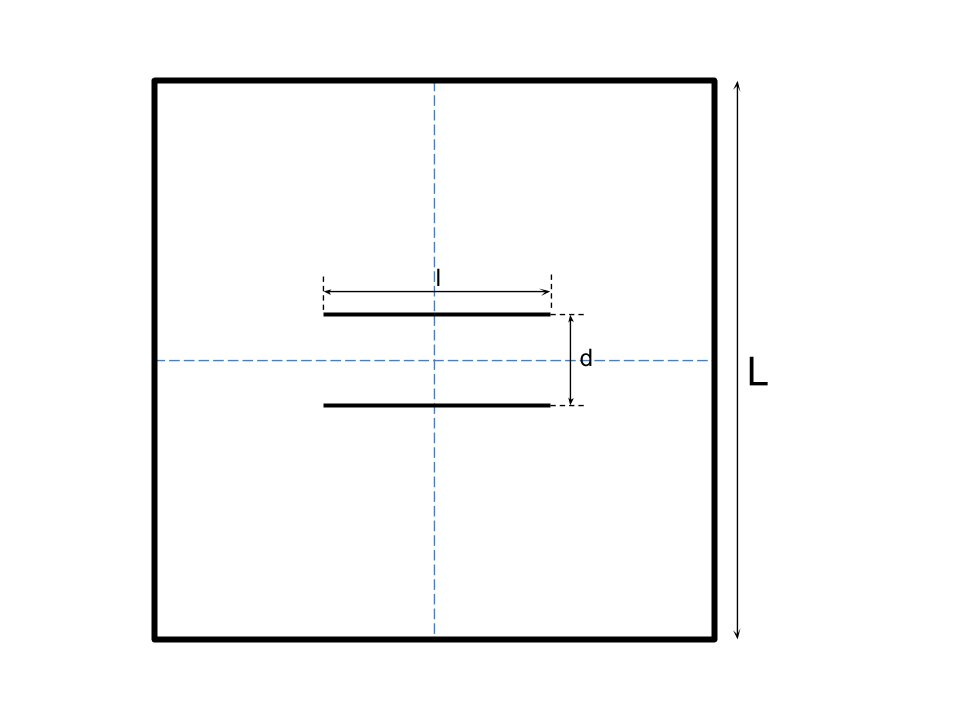
\includegraphics[width=10cm]{gridplates}
  \caption{\label{fig:gridplates} Condensador de placas paralelas.}
\end{figure}

Supongamos que existe una diferencia de potencial constante $V_0$
entre las placas (una de las placas se encuentra a $-V_0/2$ y la otra
a $V_0/2$). Adem\'as, en el borde de la regi\'on tomemos el potencial
fijo en $0$. 

El potencial el\'ectrico $V(x,y)$ en la regi\'on debe cumplir la
ecuaci\'on de Laplace 

\begin{equation*}
 \nabla^2V(x,y) = \frac{\partial^2 V(x,y)}{\partial x^2} +
 \frac{\partial^2 V(x,y)}{\partial y^2}=0. 
\end{equation*}

As\'i mismo el campo el\'ectrico est\'a dado por.
\begin{equation*}
\mathbf{E}(x,y) = -\nabla V(x,y) = \left(-\frac{\partial V(x,y)}{\partial x}, -\frac{\partial V(x,y)}{\partial y}\right)
\end{equation*}

Para calcular el potencial num\'ericamente se debe discretizar la
regi\'on como una matriz de tama\~no $L/h \times L/h$, donde $h$ es la
separaci\'on entre los puntos y utilizar el esquema de diferencias
finitas. 

Escriba un programa en C (\verb"placas.c") que encuentre el
potencial el\'ectrico con el m\'etodo de relajaci\'on usando N
iteraciones. El mismo programa debe calcular el campo el\'ectrico a
partir de la soluci\'on final del potencial.
Escriba un c\'odigo en Python \verb'grafica.py' que grafique el
potencial y el campo el\'ectrico usando \verb'imshow' y
\verb'streamplot' en una grafica llamada \verb'placas.pdf'.

Utilice $L = 5$ cm, $l = 2$ cm, $d = 1$ cm, $h = 0.02$ cm, $V_0 = 100$ V y $N = 100$ iteraciones.
 

\question{{\bf Cuerda Vibrando}}

Considere una cuerda de longitud $L$ descrita por la funci\'on
$u(x,t)$ que corresponde al desplazamiento con respecto a su
posici\'on de equilibrio. Despu\'es de una perturbaci\'on inicial, la
evoluci\'on de $u$ est\'a dada por 

\begin{equation}
\frac{\partial^2 u (x,t)}{\partial x^2} =
\frac{1}{c^2}\frac{\partial^2 u}{\partial t^2}
\end{equation}

donde $c=\sqrt{T/\rho}$ es una velocidad de propagaci\'on con $T$ la
tensi\'on de la cuerda y $\rho$ su densidad.

Las condiciones de contorno corresponden a puntos fijos.  Como
condici\'on inicial se tiene que la cuerda est\'a estirada de forma
triangular, con el m\'aximo ubicado a $8/10$ de la longitud total de
la cuerda con una altura $1$. Es decir,

\begin{equation}
u(x,t=0) = 
\begin{cases}
1.25x/L & x \leq 0.8L\\
5-5x/L & x>0.8L
\end{cases}
\end{equation}

Escriba un programa en C (\verb'cuerda.c') que resuelva esta
ecuaci\'on y encuentre $u(x,t)$. Escriba un c\'odigo en Python (\verb'animacion.py').
que produzca un gif animado (\verb'cuerda.gif') con el movimiento
resultante de la cuerda. 

Utilice $T=40$, $\rho = 10$ y $L=100$ para $0<t<200$.



\end{questions}

\end{document}

